\documentclass{article}
\usepackage[utf8]{inputenc}
\usepackage[spanish]{babel}
\usepackage{listings}
\usepackage{graphicx}
\graphicspath{ {images/} }
\usepackage{cite}

\begin{document}

\begin{titlepage}
    \begin{center}
        \vspace*{1cm}
            
        \Huge
        \textbf{Proyecto de investigación.}
            
        \vspace{0.5cm}
        \LARGE
        Taller de memoria del computador.
            
        \vspace{1.5cm}
            
        \textbf{Nicoll Caroline Chazatar Yampuezan}
            
        \vfill
            
        \vspace{0.8cm}
            
        \Large
        Despartamento de Ingeniería Electrónica y Telecomunicaciones\\
        Universidad de Antioquia\\
        Medellín\\
        Septiembre de 2020
            
    \end{center}
\end{titlepage}

\tableofcontents

\section{Sección introductoria}Para ser un buen programador en principio es esencial saber de qué manera actúa el computador cada vez que se le ordena una instrucción, es decir, conocer parte del software del computador de aquella acción, cual es el tipo de memoria en el que se guardan los archivos de cualquier tipo creado y/o modificado. Es por ello que en este documento se presenta las respuestas a las preguntas fundamentales que se debe conocer antes de iniciar a programar en cualquier tipo de lenguaje (Python, C, C++, Java, etc.), respuestas que han sido logradas gracias a una previa lectura acerca de cómo funciona la memoria del computador, lo que sucede cada vez que el usuario ordena una instrucción y conceptos sobre los diferentes tipos de memoria presentes en un computador.

\section{Sección de contenido} \label{contenido}
A partir del documento del profesor de informática II, Augusto Salazar, del semestre 2020-1. \cite{Salazar},se pudo dar respuesta a las cuatro siguientes preguntas  personales que son indispensables antes de empezar a programar en cualquier tipo de lenguaje para crear un programa o cualquier tipo de proyecto.\\


\textbf {\textit{ 1. Defina que es la memoria del computador.}}\\
La memoria del computador es el dispositivo con capacidad limitada de almacenamiento temporal de información, instrucciones y/o datos,  permitiendo que se lleven a cabo la mayoría de instrucciones ordenadas por el usuario al computador con la ayuda de controladores y microprocesadores logrando así procesar información y/o datos  para obtener resultados esperados.\\

\textbf {\textit{2. Mencione los tipos de memoria que conoce y haga una pequeña descripción de cada tipo.}}\\
Los tipos de memoria que conozco son: \\

\textit{Memoria DRAM:}\\ 
La memoria DRAM (Dynamic Random Access Memory) está formada por celdas de bits (0 o 1) distribuidas en una grilla bidimensional. Esta memoria es de acceso aleatorio que almacena temporalmente programas y datos a los que necesita acceder de forma rápida y eliminando aquellos datos y programas cuando ya no se hace uso de estos, como esta acción se realiza una y otra vez es por esto que se considera dinámica. Esta memoria posee una menor velocidad que la memoria cache pero posee mayor almacenamiento y al ser más rápida que el disco duro se convierte en ideal a la hora de trabajar.\\

\textit{Memoria ROM:}\\ 
La memoria ROM (Read Only Memory) es de solo lectura y que no permite sobre-escritura ni tampoco es de almacenamiento temporal. En ella se almacena la configuración del sistema operativo y que mantiene intacta esta información.\\

\textit{Memoria SAM:}\\ 
En la memoria SAM (Serial Acces Memory), se almacenan los datos de forma secuencial, es decir, un dato después de otro, a los cuales solo se puede acceder pasando por todos los datos anteriores que se presenten hasta llegar al requerido.\\

\textit{Memoria Cache:}\\ 
La memoria cache al igual que la RAM es de almacenamiento temporal pero como es memoria estática posee una mayor velocidad y es por esto que  con ella se trabajan los datos e instrucciones que el microprocesador usa con mayor frecuencia, se divide en 3 niveles, L1 que tiene mayor velocidad pero el menor almacenamiento que los demás niveles, L2 posee menor velocidad que L1 pero mayor almacenamiento y al igual que L1 se encuentra dentro del microprocesador y L3 que es la más lenta de las 3, pero posee mayor almacenamiento que las anteriores pero no tanta como la memoria RAM y se encuentra instalada en la placa madre.\\

\textit{Memoria Virtual:}\\ 
La memoria virtual es parte del disco duro que cumple como única función la de sostener temporalmente partes suficientes de los programas y datos que se encuentra en ejecución, estás partes ocupan espacio innecesario en la memoria RAM,  pero están listos por si el usuario llega a requerirlos y que es utilizada también cuando la memoria RAM esta llena.\\

\textit{Disco Duro:}\\ 
El disco duro tiene una gran capacidad de almacenamiento, en él se encuentra todo tipo de información que le agregamos al computador y aquella que debe almacenar para que el computador funcione como tal, es el que posee menor velocidad respecto a cualquier otro tipo de memoria debido a la rotación que debe ejercer este para poder trabajar.\\


\textbf {\textit{3. Describa la manera como se gestiona la memoria en un computador.}}\\
Una vez encendido el computador y cargado el sistema operativo en la memoria (el cual permanece cargado todo el tiempo mientas el computador este encendido), cada vez que se abre un archivo o programa, la instrucción es llevada a la memoria para que el microprocesador la tome y se encargue de buscar lo solicitado en el disco duro e inmediatamente la instrucción es eliminada o liberada de la memoria para dar lugar a otros datos, luego se carga una copia de los archivos y/o programas solicitados por el usuario en la memoria y cada modificación que se realice en  estos es una instrucción que llega a la memoria pero que es eliminada en cuanto el microprocesador la recibe, como la memoria es un espacio de almacenamiento temporal este no guarda nada hasta que es el mismo usuario quien da la orden de guardar el archivo para que sea almacenado en el disco duro y finalmente si es cerrado el programa o archivo en el que se haya estado trabajando este desparece de la memoria mas no del disco duro de manera que se podrá acceder las veces que se desee el usuario.\\
Es así entonces como la memoria actúa con datos y programas aleatorios que se están utilizando y aquellos con los que no los elimina con el fin de liberar espacio para dar lugar a nuevas instrucciones o programas que lo necesiten.
En la figura (\ref{fig:RAM.jpg}) , se muestra como es fisicamente una memoria RAM.

\begin{figure}[h]
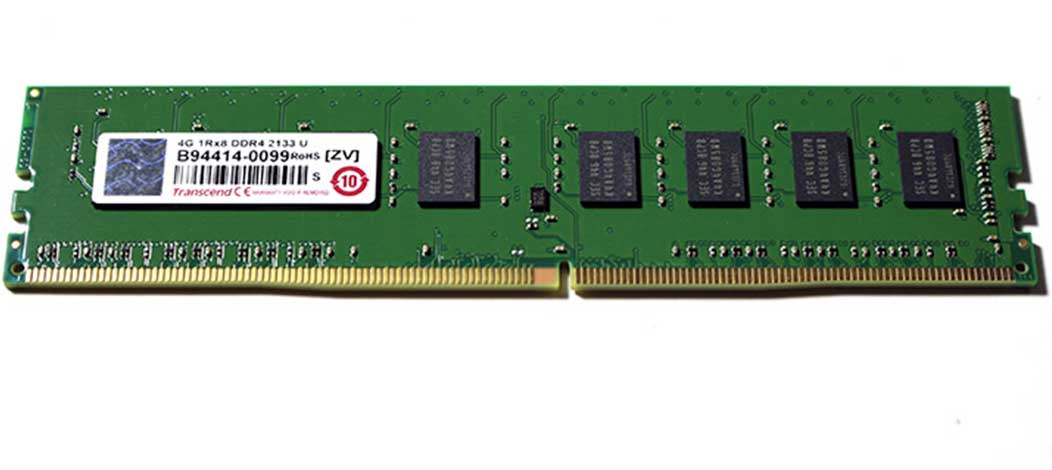
\includegraphics[width=4cm]{RAM.jpg}
\centering
\caption{Memoria RAM DDR4\cite{RAMwebsite}}
\label{fig:RAM.jpg}
\end{figure}


\textbf {\textit{4. ¿Qué hace que una memoria sea más rápida que otra? ¿Por qué esto es importante?}}\\
Lo que permite a una memoria ser más rápida que otra es la cantidad de núcleos ya que se puede lograr mucho por los ciclos que se presentan en cada uno, lo que incluye que posea más transistores y condensadores, la velocidad que posee una memoria es muy importante porque es la que permite trabajar de la manera más eficiente, logrando un buen rendimiento, y se tendrá más tiempo para avanzar o hacer otras tareas pendientes que requieran mayor almacenamiento de memoria para así quizá trabajar de la mejor manera.

\begin{lstlisting}
    
\end{lstlisting}

\section{Conclusiones} \label{conclulsion}
- La memoria del computador es aquella que permite obtener los resultados esperados a cada orden que se pide en el menor tiempo que a esta le es permitido gracias a que esta constituida por celdas.\\

- Gracias a los diferentes tipos de memoria existentes hoy en día, es posible llevar a cabo grandes proyectos de manera eficiente y segura.\\

- El adquirir el conocimiento de cómo funciona internamente el computador en cada transferencia de datos, permite estar en disposición de continuar con un buen aprendizaje como programador.

\bibliographystyle{IEEEtran}
\bibliography{references}

\end{document}
